\documentclass[1p]{elsarticle_modified}
%\bibliographystyle{elsarticle-num}

%\usepackage[colorlinks]{hyperref}
%\usepackage{abbrmath_seonhwa} %\Abb, \Ascr, \Acal ,\Abf, \Afrak
\usepackage{amsfonts}
\usepackage{amssymb}
\usepackage{amsmath}
\usepackage{amsthm}
\usepackage{scalefnt}
\usepackage{amsbsy}
\usepackage{kotex}
\usepackage{caption}
\usepackage{subfig}
\usepackage{color}
\usepackage{graphicx}
\usepackage{xcolor} %% white, black, red, green, blue, cyan, magenta, yellow
\usepackage{float}
\usepackage{setspace}
\usepackage{hyperref}

\usepackage{tikz}
\usetikzlibrary{arrows}

\usepackage{multirow}
\usepackage{array} % fixed length table
\usepackage{hhline}

%%%%%%%%%%%%%%%%%%%%%
\makeatletter
\renewcommand*\env@matrix[1][\arraystretch]{%
	\edef\arraystretch{#1}%
	\hskip -\arraycolsep
	\let\@ifnextchar\new@ifnextchar
	\array{*\c@MaxMatrixCols c}}
\makeatother %https://tex.stackexchange.com/questions/14071/how-can-i-increase-the-line-spacing-in-a-matrix
%%%%%%%%%%%%%%%

\usepackage[normalem]{ulem}

\newcommand{\msout}[1]{\ifmmode\text{\sout{\ensuremath{#1}}}\else\sout{#1}\fi}
%SOURCE: \msout is \stkout macro in https://tex.stackexchange.com/questions/20609/strikeout-in-math-mode

\newcommand{\cancel}[1]{
	\ifmmode
	{\color{red}\msout{#1}}
	\else
	{\color{red}\sout{#1}}
	\fi
}

\newcommand{\add}[1]{
	{\color{blue}\uwave{#1}}
}

\newcommand{\replace}[2]{
	\ifmmode
	{\color{red}\msout{#1}}{\color{blue}\uwave{#2}}
	\else
	{\color{red}\sout{#1}}{\color{blue}\uwave{#2}}
	\fi
}

\newcommand{\Sol}{\mathcal{S}} %segment
\newcommand{\D}{D} %diagram
\newcommand{\A}{\mathcal{A}} %arc


%%%%%%%%%%%%%%%%%%%%%%%%%%%%%5 test

\def\sl{\operatorname{\textup{SL}}(2,\Cbb)}
\def\psl{\operatorname{\textup{PSL}}(2,\Cbb)}
\def\quan{\mkern 1mu \triangleright \mkern 1mu}

\theoremstyle{definition}
\newtheorem{thm}{Theorem}[section]
\newtheorem{prop}[thm]{Proposition}
\newtheorem{lem}[thm]{Lemma}
\newtheorem{ques}[thm]{Question}
\newtheorem{cor}[thm]{Corollary}
\newtheorem{defn}[thm]{Definition}
\newtheorem{exam}[thm]{Example}
\newtheorem{rmk}[thm]{Remark}
\newtheorem{alg}[thm]{Algorithm}

\newcommand{\I}{\sqrt{-1}}
\begin{document}

%\begin{frontmatter}
%
%\title{Boundary parabolic representations of knots up to 8 crossings}
%
%%% Group authors per affiliation:
%\author{Yunhi Cho} 
%\address{Department of Mathematics, University of Seoul, Seoul, Korea}
%\ead{yhcho@uos.ac.kr}
%
%
%\author{Seonhwa Kim} %\fnref{s_kim}}
%\address{Center for Geometry and Physics, Institute for Basic Science, Pohang, 37673, Korea}
%\ead{ryeona17@ibs.re.kr}
%
%\author{Hyuk Kim}
%\address{Department of Mathematical Sciences, Seoul National University, Seoul 08826, Korea}
%\ead{hyukkim@snu.ac.kr}
%
%\author{Seokbeom Yoon}
%\address{Department of Mathematical Sciences, Seoul National University, Seoul, 08826,  Korea}
%\ead{sbyoon15@snu.ac.kr}
%
%\begin{abstract}
%We find all boundary parabolic representation of knots up to 8 crossings.
%
%\end{abstract}
%\begin{keyword}
%    \MSC[2010] 57M25 
%\end{keyword}
%
%\end{frontmatter}

%\linenumbers
%\tableofcontents
%
\newcommand\colored[1]{\textcolor{white}{\rule[-0.35ex]{0.8em}{1.4ex}}\kern-0.8em\color{red} #1}%
%\newcommand\colored[1]{\textcolor{white}{ #1}\kern-2.17ex	\textcolor{white}{ #1}\kern-1.81ex	\textcolor{white}{ #1}\kern-2.15ex\color{red}#1	}

{\Large $\underline{12a_{0024}~(K12a_{0024})}$}

\setlength{\tabcolsep}{10pt}
\renewcommand{\arraystretch}{1.6}
\vspace{1cm}\begin{tabular}{m{100pt}>{\centering\arraybackslash}m{274pt}}
\multirow{5}{120pt}{
	\centering
	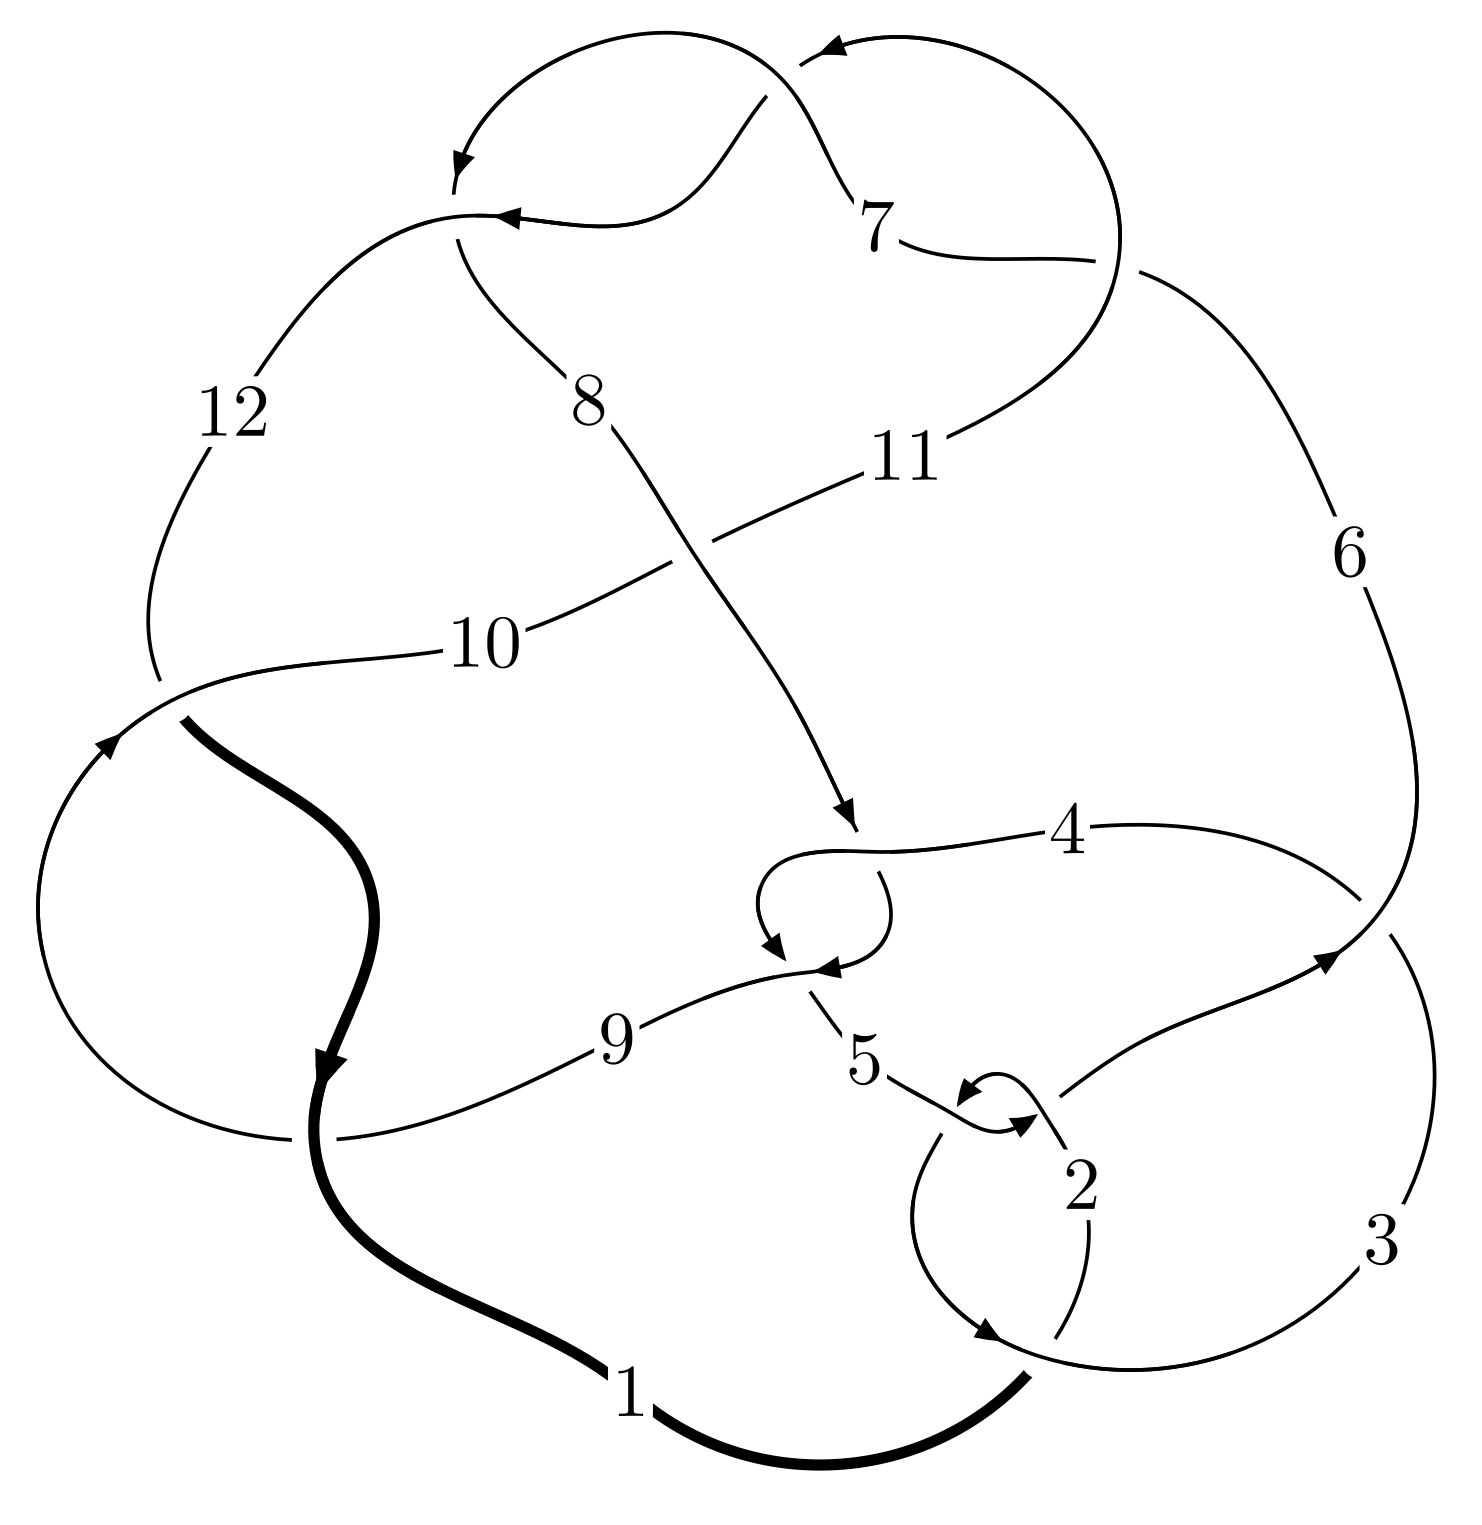
\includegraphics[width=112pt]{../../../GIT/diagram.site/Diagrams/png/825_12a_0024.png}\\
\ \ \ A knot diagram\footnotemark}&
\allowdisplaybreaks
\textbf{Linearized knot diagam} \\
\cline{2-2}
 &
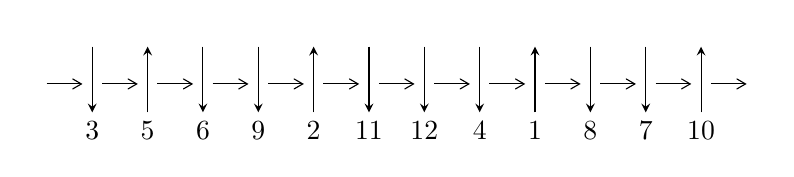
\begin{tikzpicture}[x=20pt, y=17pt]
	% nodes
	\node (C0) at (0, 0) {};
	\node (C1) at (1, 0) {};
	\node (C1U) at (1, +1) {};
	\node (C1D) at (1, -1) {3};

	\node (C2) at (2, 0) {};
	\node (C2U) at (2, +1) {};
	\node (C2D) at (2, -1) {5};

	\node (C3) at (3, 0) {};
	\node (C3U) at (3, +1) {};
	\node (C3D) at (3, -1) {6};

	\node (C4) at (4, 0) {};
	\node (C4U) at (4, +1) {};
	\node (C4D) at (4, -1) {9};

	\node (C5) at (5, 0) {};
	\node (C5U) at (5, +1) {};
	\node (C5D) at (5, -1) {2};

	\node (C6) at (6, 0) {};
	\node (C6U) at (6, +1) {};
	\node (C6D) at (6, -1) {11};

	\node (C7) at (7, 0) {};
	\node (C7U) at (7, +1) {};
	\node (C7D) at (7, -1) {12};

	\node (C8) at (8, 0) {};
	\node (C8U) at (8, +1) {};
	\node (C8D) at (8, -1) {4};

	\node (C9) at (9, 0) {};
	\node (C9U) at (9, +1) {};
	\node (C9D) at (9, -1) {1};

	\node (C10) at (10, 0) {};
	\node (C10U) at (10, +1) {};
	\node (C10D) at (10, -1) {8};

	\node (C11) at (11, 0) {};
	\node (C11U) at (11, +1) {};
	\node (C11D) at (11, -1) {7};

	\node (C12) at (12, 0) {};
	\node (C12U) at (12, +1) {};
	\node (C12D) at (12, -1) {10};
	\node (C13) at (13, 0) {};

	% arrows
	\draw[->,>={angle 60}]
	(C0) edge (C1) (C1) edge (C2) (C2) edge (C3) (C3) edge (C4) (C4) edge (C5) (C5) edge (C6) (C6) edge (C7) (C7) edge (C8) (C8) edge (C9) (C9) edge (C10) (C10) edge (C11) (C11) edge (C12) (C12) edge (C13) ;	\draw[->,>=stealth]
	(C1U) edge (C1D) (C2D) edge (C2U) (C3U) edge (C3D) (C4U) edge (C4D) (C5D) edge (C5U) (C6U) edge (C6D) (C7U) edge (C7D) (C8U) edge (C8D) (C9D) edge (C9U) (C10U) edge (C10D) (C11U) edge (C11D) (C12D) edge (C12U) ;
	\end{tikzpicture} \\
\hhline{~~} \\& 
\textbf{Solving Sequence} \\ \cline{2-2} 
 &
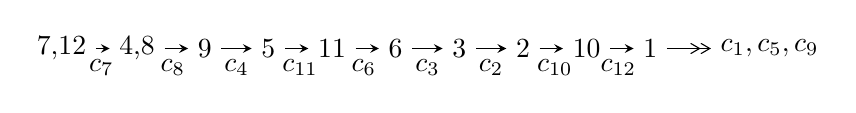
\begin{tikzpicture}[x=23pt, y=7pt]
	% node
	\node (A0) at (-1/8, 0) {7,12};
	\node (A1) at (17/16, 0) {4,8};
	\node (A2) at (17/8, 0) {9};
	\node (A3) at (25/8, 0) {5};
	\node (A4) at (33/8, 0) {11};
	\node (A5) at (41/8, 0) {6};
	\node (A6) at (49/8, 0) {3};
	\node (A7) at (57/8, 0) {2};
	\node (A8) at (65/8, 0) {10};
	\node (A9) at (73/8, 0) {1};
	\node (C1) at (1/2, -1) {$c_{7}$};
	\node (C2) at (13/8, -1) {$c_{8}$};
	\node (C3) at (21/8, -1) {$c_{4}$};
	\node (C4) at (29/8, -1) {$c_{11}$};
	\node (C5) at (37/8, -1) {$c_{6}$};
	\node (C6) at (45/8, -1) {$c_{3}$};
	\node (C7) at (53/8, -1) {$c_{2}$};
	\node (C8) at (61/8, -1) {$c_{10}$};
	\node (C9) at (69/8, -1) {$c_{12}$};
	\node (A10) at (11, 0) {$c_{1},c_{5},c_{9}$};

	% edge
	\draw[->,>=stealth]	
	(A0) edge (A1) (A1) edge (A2) (A2) edge (A3) (A3) edge (A4) (A4) edge (A5) (A5) edge (A6) (A6) edge (A7) (A7) edge (A8) (A8) edge (A9) ;
	\draw[->>,>={angle 60}]	
	(A9) edge (A10);
\end{tikzpicture} \\ 

\end{tabular} \\

\footnotetext{
The image of knot diagram is generated by the software ``\textbf{Draw programme}" developed by Andrew Bartholomew(\url{http://www.layer8.co.uk/maths/draw/index.htm\#Running-draw}), where we modified some parts for our purpose(\url{https://github.com/CATsTAILs/LinksPainter}).
}\phantom \\ \newline 
\centering \textbf{Ideals for irreducible components\footnotemark of $X_{\text{par}}$} 
 
\begin{align*}
I^u_{1}&=\langle 
17 u^{89}-27 u^{88}+\cdots+2 b+10,\;11 u^{89}-17 u^{88}+\cdots+2 a+9,\;u^{90}-3 u^{89}+\cdots-2 u-1\rangle \\
I^u_{2}&=\langle 
- u^2 a+b,\;u^4 a+u^3 a- u^2 a+a^2- a u+u^2+u-1,\;u^5+u^4-2 u^3- u^2+u-1\rangle \\
\\
\end{align*}
\raggedright * 2 irreducible components of $\dim_{\mathbb{C}}=0$, with total 100 representations.\\
\footnotetext{All coefficients of polynomials are rational numbers. But the coefficients are sometimes approximated in decimal forms when there is not enough margin.}
\newpage
\renewcommand{\arraystretch}{1}
\centering \section*{I. $I^u_{1}= \langle 17 u^{89}-27 u^{88}+\cdots+2 b+10,\;11 u^{89}-17 u^{88}+\cdots+2 a+9,\;u^{90}-3 u^{89}+\cdots-2 u-1 \rangle$}
\flushleft \textbf{(i) Arc colorings}\\
\begin{tabular}{m{7pt} m{180pt} m{7pt} m{180pt} }
\flushright $a_{7}=$&$\begin{pmatrix}1\\0\end{pmatrix}$ \\
\flushright $a_{12}=$&$\begin{pmatrix}0\\u\end{pmatrix}$ \\
\flushright $a_{4}=$&$\begin{pmatrix}-\frac{11}{2} u^{89}+\frac{17}{2} u^{88}+\cdots-\frac{13}{2} u-\frac{9}{2}\\-\frac{17}{2} u^{89}+\frac{27}{2} u^{88}+\cdots-\frac{27}{2} u-5\end{pmatrix}$ \\
\flushright $a_{8}=$&$\begin{pmatrix}1\\u^2\end{pmatrix}$ \\
\flushright $a_{9}=$&$\begin{pmatrix}- u^{11}+6 u^9-12 u^7+8 u^5- u^3+2 u\\- u^{13}+5 u^{11}-7 u^9+2 u^5+3 u^3+u\end{pmatrix}$ \\
\flushright $a_{5}=$&$\begin{pmatrix}\frac{3}{2} u^{89}-\frac{1}{2} u^{88}+\cdots+\frac{15}{2} u+\frac{1}{2}\\\frac{9}{2} u^{89}-\frac{9}{2} u^{88}+\cdots+\frac{15}{2} u+3\end{pmatrix}$ \\
\flushright $a_{11}=$&$\begin{pmatrix}u\\u\end{pmatrix}$ \\
\flushright $a_{6}=$&$\begin{pmatrix}- u^2+1\\- u^2\end{pmatrix}$ \\
\flushright $a_{3}=$&$\begin{pmatrix}-2 u^{89}+4 u^{88}+\cdots+2 u-\frac{3}{2}\\-2 u^{89}+4 u^{88}+\cdots-\frac{5}{2} u-1\end{pmatrix}$ \\
\flushright $a_{2}=$&$\begin{pmatrix}\frac{1}{2} u^{86}-\frac{1}{2} u^{85}+\cdots+5 u-\frac{3}{2}\\- u^{89}+2 u^{88}+\cdots-\frac{1}{2} u-1\end{pmatrix}$ \\
\flushright $a_{10}=$&$\begin{pmatrix}- u^3+2 u\\- u^5+u^3+u\end{pmatrix}$ \\
\flushright $a_{1}=$&$\begin{pmatrix}u^7-4 u^5+4 u^3\\u^9-3 u^7+u^5+2 u^3+u\end{pmatrix}$\\&\end{tabular}
\flushleft \textbf{(ii) Obstruction class $= -1$}\\~\\
\flushleft \textbf{(iii) Cusp Shapes $= \frac{5}{2} u^{89}-\frac{7}{2} u^{88}+\cdots+\frac{35}{2} u+\frac{3}{2}$}\\~\\
\newpage\renewcommand{\arraystretch}{1}
\flushleft \textbf{(iv) u-Polynomials at the component}\newline \\
\begin{tabular}{m{50pt}|m{274pt}}
Crossings & \hspace{64pt}u-Polynomials at each crossing \\
\hline $$\begin{aligned}c_{1}\end{aligned}$$&$\begin{aligned}
&u^{90}+46 u^{89}+\cdots+5 u+1
\end{aligned}$\\
\hline $$\begin{aligned}c_{2},c_{5}\end{aligned}$$&$\begin{aligned}
&u^{90}+6 u^{89}+\cdots+7 u+1
\end{aligned}$\\
\hline $$\begin{aligned}c_{3}\end{aligned}$$&$\begin{aligned}
&u^{90}-6 u^{89}+\cdots-21049 u+2857
\end{aligned}$\\
\hline $$\begin{aligned}c_{4},c_{8}\end{aligned}$$&$\begin{aligned}
&u^{90}- u^{89}+\cdots-1024 u-1024
\end{aligned}$\\
\hline $$\begin{aligned}c_{6},c_{7},c_{11}\end{aligned}$$&$\begin{aligned}
&u^{90}+3 u^{89}+\cdots+2 u-1
\end{aligned}$\\
\hline $$\begin{aligned}c_{9},c_{12}\end{aligned}$$&$\begin{aligned}
&u^{90}+13 u^{89}+\cdots+250 u-7
\end{aligned}$\\
\hline $$\begin{aligned}c_{10}\end{aligned}$$&$\begin{aligned}
&u^{90}-9 u^{89}+\cdots-5322 u+1237
\end{aligned}$\\
\hline
\end{tabular}\\~\\
\newpage\renewcommand{\arraystretch}{1}
\flushleft \textbf{(v) Riley Polynomials at the component}\newline \\
\begin{tabular}{m{50pt}|m{274pt}}
Crossings & \hspace{64pt}Riley Polynomials at each crossing \\
\hline $$\begin{aligned}c_{1}\end{aligned}$$&$\begin{aligned}
&y^{90}+2 y^{89}+\cdots-19 y+1
\end{aligned}$\\
\hline $$\begin{aligned}c_{2},c_{5}\end{aligned}$$&$\begin{aligned}
&y^{90}+46 y^{89}+\cdots+5 y+1
\end{aligned}$\\
\hline $$\begin{aligned}c_{3}\end{aligned}$$&$\begin{aligned}
&y^{90}-42 y^{89}+\cdots+178045685 y+8162449
\end{aligned}$\\
\hline $$\begin{aligned}c_{4},c_{8}\end{aligned}$$&$\begin{aligned}
&y^{90}-55 y^{89}+\cdots-16777216 y+1048576
\end{aligned}$\\
\hline $$\begin{aligned}c_{6},c_{7},c_{11}\end{aligned}$$&$\begin{aligned}
&y^{90}-85 y^{89}+\cdots-2 y+1
\end{aligned}$\\
\hline $$\begin{aligned}c_{9},c_{12}\end{aligned}$$&$\begin{aligned}
&y^{90}+79 y^{89}+\cdots-113894 y+49
\end{aligned}$\\
\hline $$\begin{aligned}c_{10}\end{aligned}$$&$\begin{aligned}
&y^{90}-33 y^{89}+\cdots-33961930 y+1530169
\end{aligned}$\\
\hline
\end{tabular}\\~\\
\newpage\flushleft \textbf{(vi) Complex Volumes and Cusp Shapes}
$$\begin{array}{c|c|c}  
\text{Solutions to }I^u_{1}& \I (\text{vol} + \sqrt{-1}CS) & \text{Cusp shape}\\
 \hline 
\begin{aligned}
u &= \phantom{-}1.035540 + 0.147829 I \\
a &= -1.178990 + 0.129145 I \\
b &= -2.35944 + 0.04325 I\end{aligned}
 & -4.04276 + 3.69637 I & \phantom{-0.000000 } 0 \\ \hline\begin{aligned}
u &= \phantom{-}1.035540 - 0.147829 I \\
a &= -1.178990 - 0.129145 I \\
b &= -2.35944 - 0.04325 I\end{aligned}
 & -4.04276 - 3.69637 I & \phantom{-0.000000 } 0 \\ \hline\begin{aligned}
u &= \phantom{-}1.159310 + 0.090200 I \\
a &= \phantom{-}0.799616 - 0.379304 I \\
b &= \phantom{-}1.82834 - 0.69618 I\end{aligned}
 & -1.75007 - 0.25828 I & \phantom{-0.000000 } 0 \\ \hline\begin{aligned}
u &= \phantom{-}1.159310 - 0.090200 I \\
a &= \phantom{-}0.799616 + 0.379304 I \\
b &= \phantom{-}1.82834 + 0.69618 I\end{aligned}
 & -1.75007 + 0.25828 I & \phantom{-0.000000 } 0 \\ \hline\begin{aligned}
u &= -0.437999 + 0.686714 I \\
a &= \phantom{-}0.33190 - 1.91263 I \\
b &= \phantom{-}0.196118 - 0.060111 I\end{aligned}
 & -9.70066 + 3.66881 I & -11.15932 - 3.34519 I \\ \hline\begin{aligned}
u &= -0.437999 - 0.686714 I \\
a &= \phantom{-}0.33190 + 1.91263 I \\
b &= \phantom{-}0.196118 + 0.060111 I\end{aligned}
 & -9.70066 - 3.66881 I & -11.15932 + 3.34519 I \\ \hline\begin{aligned}
u &= -0.408798 + 0.704111 I \\
a &= \phantom{-}0.19713 - 2.43169 I \\
b &= -0.1107110 + 0.0409626 I\end{aligned}
 & -7.6515 + 12.5202 I & -8.50844 - 9.24171 I \\ \hline\begin{aligned}
u &= -0.408798 - 0.704111 I \\
a &= \phantom{-}0.19713 + 2.43169 I \\
b &= -0.1107110 - 0.0409626 I\end{aligned}
 & -7.6515 - 12.5202 I & -8.50844 + 9.24171 I \\ \hline\begin{aligned}
u &= -0.519185 + 0.621006 I \\
a &= -0.639891 + 0.342871 I \\
b &= -1.157860 + 0.042784 I\end{aligned}
 & -10.00680 + 0.68806 I & -11.88470 - 2.78683 I \\ \hline\begin{aligned}
u &= -0.519185 - 0.621006 I \\
a &= -0.639891 - 0.342871 I \\
b &= -1.157860 - 0.042784 I\end{aligned}
 & -10.00680 - 0.68806 I & -11.88470 + 2.78683 I\\
 \hline 
 \end{array}$$\newpage$$\begin{array}{c|c|c}  
\text{Solutions to }I^u_{1}& \I (\text{vol} + \sqrt{-1}CS) & \text{Cusp shape}\\
 \hline 
\begin{aligned}
u &= -0.551816 + 0.587844 I \\
a &= -0.721885 - 0.251112 I \\
b &= -1.50250 - 0.11783 I\end{aligned}
 & -8.18869 - 8.18776 I & -9.87272 + 3.39708 I \\ \hline\begin{aligned}
u &= -0.551816 - 0.587844 I \\
a &= -0.721885 + 0.251112 I \\
b &= -1.50250 + 0.11783 I\end{aligned}
 & -8.18869 + 8.18776 I & -9.87272 - 3.39708 I \\ \hline\begin{aligned}
u &= -0.411438 + 0.688379 I \\
a &= -0.04849 + 2.23057 I \\
b &= -0.0163093 - 0.1154220 I\end{aligned}
 & -4.87794 + 7.26864 I & -5.96969 - 5.95912 I \\ \hline\begin{aligned}
u &= -0.411438 - 0.688379 I \\
a &= -0.04849 - 2.23057 I \\
b &= -0.0163093 + 0.1154220 I\end{aligned}
 & -4.87794 - 7.26864 I & -5.96969 + 5.95912 I \\ \hline\begin{aligned}
u &= -0.527543 + 0.586369 I \\
a &= \phantom{-}0.466491 + 0.096694 I \\
b &= \phantom{-}1.329780 + 0.182524 I\end{aligned}
 & -5.33184 - 3.01556 I & -7.21234 - 0.07113 I \\ \hline\begin{aligned}
u &= -0.527543 - 0.586369 I \\
a &= \phantom{-}0.466491 - 0.096694 I \\
b &= \phantom{-}1.329780 - 0.182524 I\end{aligned}
 & -5.33184 + 3.01556 I & -7.21234 + 0.07113 I \\ \hline\begin{aligned}
u &= \phantom{-}0.426107 + 0.647594 I \\
a &= \phantom{-}1.24151 - 1.36025 I \\
b &= \phantom{-}0.698493 - 0.178607 I\end{aligned}
 & -4.09139 - 5.96624 I & -8.21287 + 6.74869 I \\ \hline\begin{aligned}
u &= \phantom{-}0.426107 - 0.647594 I \\
a &= \phantom{-}1.24151 + 1.36025 I \\
b &= \phantom{-}0.698493 + 0.178607 I\end{aligned}
 & -4.09139 + 5.96624 I & -8.21287 - 6.74869 I \\ \hline\begin{aligned}
u &= \phantom{-}0.469022 + 0.601759 I \\
a &= \phantom{-}0.73660 - 1.53917 I \\
b &= \phantom{-}0.609093 - 0.543821 I\end{aligned}
 & -4.28017 + 1.86136 I & -8.94738 - 0.21875 I \\ \hline\begin{aligned}
u &= \phantom{-}0.469022 - 0.601759 I \\
a &= \phantom{-}0.73660 + 1.53917 I \\
b &= \phantom{-}0.609093 + 0.543821 I\end{aligned}
 & -4.28017 - 1.86136 I & -8.94738 + 0.21875 I\\
 \hline 
 \end{array}$$\newpage$$\begin{array}{c|c|c}  
\text{Solutions to }I^u_{1}& \I (\text{vol} + \sqrt{-1}CS) & \text{Cusp shape}\\
 \hline 
\begin{aligned}
u &= \phantom{-}0.730493 + 0.189798 I \\
a &= -0.774454 - 0.466152 I \\
b &= -1.39580 - 0.61388 I\end{aligned}
 & -4.18196 - 3.80025 I & -10.98096 + 4.73672 I \\ \hline\begin{aligned}
u &= \phantom{-}0.730493 - 0.189798 I \\
a &= -0.774454 + 0.466152 I \\
b &= -1.39580 + 0.61388 I\end{aligned}
 & -4.18196 + 3.80025 I & -10.98096 - 4.73672 I \\ \hline\begin{aligned}
u &= -0.413257 + 0.622880 I \\
a &= \phantom{-}0.73526 + 1.38556 I \\
b &= -0.463774 - 0.507608 I\end{aligned}
 & -1.76351 + 4.66487 I & -7.53917 - 7.21944 I \\ \hline\begin{aligned}
u &= -0.413257 - 0.622880 I \\
a &= \phantom{-}0.73526 - 1.38556 I \\
b &= -0.463774 + 0.507608 I\end{aligned}
 & -1.76351 - 4.66487 I & -7.53917 + 7.21944 I \\ \hline\begin{aligned}
u &= -0.433709 + 0.592654 I \\
a &= -0.735605 - 0.677095 I \\
b &= \phantom{-}0.768130 + 0.537666 I\end{aligned}
 & -1.87712 - 0.73957 I & -8.41694 - 0.27201 I \\ \hline\begin{aligned}
u &= -0.433709 - 0.592654 I \\
a &= -0.735605 + 0.677095 I \\
b &= \phantom{-}0.768130 - 0.537666 I\end{aligned}
 & -1.87712 + 0.73957 I & -8.41694 + 0.27201 I \\ \hline\begin{aligned}
u &= \phantom{-}1.261540 + 0.134061 I \\
a &= \phantom{-}0.602278 - 0.940882 I \\
b &= \phantom{-}1.76416 - 1.98860 I\end{aligned}
 & -1.67033 - 1.06008 I & \phantom{-0.000000 } 0 \\ \hline\begin{aligned}
u &= \phantom{-}1.261540 - 0.134061 I \\
a &= \phantom{-}0.602278 + 0.940882 I \\
b &= \phantom{-}1.76416 + 1.98860 I\end{aligned}
 & -1.67033 + 1.06008 I & \phantom{-0.000000 } 0 \\ \hline\begin{aligned}
u &= \phantom{-}0.409031 + 0.601690 I \\
a &= -0.89429 + 1.09608 I \\
b &= -0.448688 + 0.262318 I\end{aligned}
 & -1.22702 - 1.91248 I & -3.96230 + 3.55807 I \\ \hline\begin{aligned}
u &= \phantom{-}0.409031 - 0.601690 I \\
a &= -0.89429 - 1.09608 I \\
b &= -0.448688 - 0.262318 I\end{aligned}
 & -1.22702 + 1.91248 I & -3.96230 - 3.55807 I\\
 \hline 
 \end{array}$$\newpage$$\begin{array}{c|c|c}  
\text{Solutions to }I^u_{1}& \I (\text{vol} + \sqrt{-1}CS) & \text{Cusp shape}\\
 \hline 
\begin{aligned}
u &= -1.276300 + 0.096082 I \\
a &= \phantom{-}1.40005 + 1.66428 I \\
b &= \phantom{-}2.00156 + 2.73492 I\end{aligned}
 & -2.65099 - 0.98383 I & \phantom{-0.000000 } 0 \\ \hline\begin{aligned}
u &= -1.276300 - 0.096082 I \\
a &= \phantom{-}1.40005 - 1.66428 I \\
b &= \phantom{-}2.00156 - 2.73492 I\end{aligned}
 & -2.65099 + 0.98383 I & \phantom{-0.000000 } 0 \\ \hline\begin{aligned}
u &= -1.274020 + 0.144176 I \\
a &= -0.82202 - 1.79830 I \\
b &= -1.22136 - 3.06947 I\end{aligned}
 & -1.80283 + 3.89148 I & \phantom{-0.000000 } 0 \\ \hline\begin{aligned}
u &= -1.274020 - 0.144176 I \\
a &= -0.82202 + 1.79830 I \\
b &= -1.22136 + 3.06947 I\end{aligned}
 & -1.80283 - 3.89148 I & \phantom{-0.000000 } 0 \\ \hline\begin{aligned}
u &= \phantom{-}0.203863 + 0.668626 I \\
a &= \phantom{-}1.87283 + 0.93707 I \\
b &= \phantom{-}0.0335509 + 0.1254080 I\end{aligned}
 & -2.25258 + 0.41899 I & -7.65968 + 0.68972 I \\ \hline\begin{aligned}
u &= \phantom{-}0.203863 - 0.668626 I \\
a &= \phantom{-}1.87283 - 0.93707 I \\
b &= \phantom{-}0.0335509 - 0.1254080 I\end{aligned}
 & -2.25258 - 0.41899 I & -7.65968 - 0.68972 I \\ \hline\begin{aligned}
u &= \phantom{-}0.119191 + 0.683033 I \\
a &= \phantom{-}1.96671 + 1.78497 I \\
b &= -0.0552694 - 0.0778810 I\end{aligned}
 & -1.33539 - 7.02339 I & -4.65258 + 7.68511 I \\ \hline\begin{aligned}
u &= \phantom{-}0.119191 - 0.683033 I \\
a &= \phantom{-}1.96671 - 1.78497 I \\
b &= -0.0552694 + 0.0778810 I\end{aligned}
 & -1.33539 + 7.02339 I & -4.65258 - 7.68511 I \\ \hline\begin{aligned}
u &= \phantom{-}0.308931 + 0.619062 I \\
a &= -1.193670 + 0.120245 I \\
b &= -0.235643 - 0.064548 I\end{aligned}
 & -0.48363 - 2.34563 I & -5.80863 + 1.86911 I \\ \hline\begin{aligned}
u &= \phantom{-}0.308931 - 0.619062 I \\
a &= -1.193670 - 0.120245 I \\
b &= -0.235643 + 0.064548 I\end{aligned}
 & -0.48363 + 2.34563 I & -5.80863 - 1.86911 I\\
 \hline 
 \end{array}$$\newpage$$\begin{array}{c|c|c}  
\text{Solutions to }I^u_{1}& \I (\text{vol} + \sqrt{-1}CS) & \text{Cusp shape}\\
 \hline 
\begin{aligned}
u &= \phantom{-}1.307800 + 0.159281 I \\
a &= -0.482256 + 1.274220 I \\
b &= -1.78724 + 2.77159 I\end{aligned}
 & -3.40681 - 5.45128 I & \phantom{-0.000000 } 0 \\ \hline\begin{aligned}
u &= \phantom{-}1.307800 - 0.159281 I \\
a &= -0.482256 - 1.274220 I \\
b &= -1.78724 - 2.77159 I\end{aligned}
 & -3.40681 + 5.45128 I & \phantom{-0.000000 } 0 \\ \hline\begin{aligned}
u &= -1.299790 + 0.224911 I \\
a &= -0.01884 - 1.71554 I \\
b &= -0.02023 - 3.28053 I\end{aligned}
 & -3.29956 + 5.65949 I & \phantom{-0.000000 } 0 \\ \hline\begin{aligned}
u &= -1.299790 - 0.224911 I \\
a &= -0.01884 + 1.71554 I \\
b &= -0.02023 + 3.28053 I\end{aligned}
 & -3.29956 - 5.65949 I & \phantom{-0.000000 } 0 \\ \hline\begin{aligned}
u &= -1.297930 + 0.254453 I \\
a &= -0.23628 + 1.82699 I \\
b &= -0.33307 + 3.61523 I\end{aligned}
 & -5.74518 + 10.42230 I & \phantom{-0.000000 } 0 \\ \hline\begin{aligned}
u &= -1.297930 - 0.254453 I \\
a &= -0.23628 - 1.82699 I \\
b &= -0.33307 - 3.61523 I\end{aligned}
 & -5.74518 - 10.42230 I & \phantom{-0.000000 } 0 \\ \hline\begin{aligned}
u &= \phantom{-}1.343220 + 0.065105 I \\
a &= -0.086124 + 0.903621 I \\
b &= -0.56348 + 2.46276 I\end{aligned}
 & -5.00570 + 0.83074 I & \phantom{-0.000000 } 0 \\ \hline\begin{aligned}
u &= \phantom{-}1.343220 - 0.065105 I \\
a &= -0.086124 - 0.903621 I \\
b &= -0.56348 - 2.46276 I\end{aligned}
 & -5.00570 - 0.83074 I & \phantom{-0.000000 } 0 \\ \hline\begin{aligned}
u &= \phantom{-}0.114121 + 0.632819 I \\
a &= -1.51121 - 1.76847 I \\
b &= -0.0735512 + 0.0732549 I\end{aligned}
 & \phantom{-}1.09432 - 2.53863 I & -0.39286 + 4.64184 I \\ \hline\begin{aligned}
u &= \phantom{-}0.114121 - 0.632819 I \\
a &= -1.51121 + 1.76847 I \\
b &= -0.0735512 - 0.0732549 I\end{aligned}
 & \phantom{-}1.09432 + 2.53863 I & -0.39286 - 4.64184 I\\
 \hline 
 \end{array}$$\newpage$$\begin{array}{c|c|c}  
\text{Solutions to }I^u_{1}& \I (\text{vol} + \sqrt{-1}CS) & \text{Cusp shape}\\
 \hline 
\begin{aligned}
u &= -1.360390 + 0.243110 I \\
a &= -0.350565 + 1.164240 I \\
b &= -0.87333 + 2.45780 I\end{aligned}
 & -7.18925 + 2.87956 I & \phantom{-0.000000 } 0 \\ \hline\begin{aligned}
u &= -1.360390 - 0.243110 I \\
a &= -0.350565 - 1.164240 I \\
b &= -0.87333 - 2.45780 I\end{aligned}
 & -7.18925 - 2.87956 I & \phantom{-0.000000 } 0 \\ \hline\begin{aligned}
u &= -1.41779\phantom{ +0.000000I} \\
a &= \phantom{-}0.815249\phantom{ +0.000000I} \\
b &= \phantom{-}0.429776\phantom{ +0.000000I}\end{aligned}
 & -7.33492\phantom{ +0.000000I} & \phantom{-0.000000 } 0 \\ \hline\begin{aligned}
u &= \phantom{-}0.398019 + 0.418448 I \\
a &= -0.083964 + 1.026110 I \\
b &= \phantom{-}0.176209 + 0.457399 I\end{aligned}
 & -1.15580 - 0.94935 I & -8.91971 + 4.56142 I \\ \hline\begin{aligned}
u &= \phantom{-}0.398019 - 0.418448 I \\
a &= -0.083964 - 1.026110 I \\
b &= \phantom{-}0.176209 - 0.457399 I\end{aligned}
 & -1.15580 + 0.94935 I & -8.91971 - 4.56142 I \\ \hline\begin{aligned}
u &= -1.41162 + 0.17588 I \\
a &= \phantom{-}0.399227 + 0.654735 I \\
b &= \phantom{-}0.45610 + 1.60564 I\end{aligned}
 & -6.84094 + 3.22476 I & \phantom{-0.000000 } 0 \\ \hline\begin{aligned}
u &= -1.41162 - 0.17588 I \\
a &= \phantom{-}0.399227 - 0.654735 I \\
b &= \phantom{-}0.45610 - 1.60564 I\end{aligned}
 & -6.84094 - 3.22476 I & \phantom{-0.000000 } 0 \\ \hline\begin{aligned}
u &= -1.41987 + 0.23861 I \\
a &= \phantom{-}0.560750 - 0.298797 I \\
b &= \phantom{-}1.43017 - 0.55315 I\end{aligned}
 & -6.02002 + 5.49310 I & \phantom{-0.000000 } 0 \\ \hline\begin{aligned}
u &= -1.41987 - 0.23861 I \\
a &= \phantom{-}0.560750 + 0.298797 I \\
b &= \phantom{-}1.43017 + 0.55315 I\end{aligned}
 & -6.02002 - 5.49310 I & \phantom{-0.000000 } 0 \\ \hline\begin{aligned}
u &= \phantom{-}0.559261\phantom{ +0.000000I} \\
a &= \phantom{-}0.232713\phantom{ +0.000000I} \\
b &= \phantom{-}0.959638\phantom{ +0.000000I}\end{aligned}
 & -1.28839\phantom{ +0.000000I} & -8.06550\phantom{ +0.000000I}\\
 \hline 
 \end{array}$$\newpage$$\begin{array}{c|c|c}  
\text{Solutions to }I^u_{1}& \I (\text{vol} + \sqrt{-1}CS) & \text{Cusp shape}\\
 \hline 
\begin{aligned}
u &= -1.44510 + 0.02573 I \\
a &= -0.626593 - 0.164956 I \\
b &= \phantom{-}0.040468 - 0.468518 I\end{aligned}
 & -10.78930 + 4.28605 I & \phantom{-0.000000 } 0 \\ \hline\begin{aligned}
u &= -1.44510 - 0.02573 I \\
a &= -0.626593 + 0.164956 I \\
b &= \phantom{-}0.040468 + 0.468518 I\end{aligned}
 & -10.78930 - 4.28605 I & \phantom{-0.000000 } 0 \\ \hline\begin{aligned}
u &= \phantom{-}0.009036 + 0.549222 I \\
a &= -0.76604 - 2.41165 I \\
b &= -0.340171 + 0.150886 I\end{aligned}
 & \phantom{-}2.08637 - 1.40419 I & \phantom{-}2.94065 + 3.79757 I \\ \hline\begin{aligned}
u &= \phantom{-}0.009036 - 0.549222 I \\
a &= -0.76604 + 2.41165 I \\
b &= -0.340171 - 0.150886 I\end{aligned}
 & \phantom{-}2.08637 + 1.40419 I & \phantom{-}2.94065 - 3.79757 I \\ \hline\begin{aligned}
u &= -1.45603 + 0.22571 I \\
a &= \phantom{-}0.786694 + 0.252582 I \\
b &= \phantom{-}1.90775 + 1.02183 I\end{aligned}
 & -7.22826 + 4.96225 I & \phantom{-0.000000 } 0 \\ \hline\begin{aligned}
u &= -1.45603 - 0.22571 I \\
a &= \phantom{-}0.786694 - 0.252582 I \\
b &= \phantom{-}1.90775 - 1.02183 I\end{aligned}
 & -7.22826 - 4.96225 I & \phantom{-0.000000 } 0 \\ \hline\begin{aligned}
u &= \phantom{-}1.46085 + 0.21961 I \\
a &= \phantom{-}1.51400 - 0.77409 I \\
b &= \phantom{-}2.57466 - 0.64144 I\end{aligned}
 & -7.96927 - 2.24977 I & \phantom{-0.000000 } 0 \\ \hline\begin{aligned}
u &= \phantom{-}1.46085 - 0.21961 I \\
a &= \phantom{-}1.51400 + 0.77409 I \\
b &= \phantom{-}2.57466 + 0.64144 I\end{aligned}
 & -7.96927 + 2.24977 I & \phantom{-0.000000 } 0 \\ \hline\begin{aligned}
u &= \phantom{-}1.45954 + 0.23127 I \\
a &= -1.53208 + 1.18300 I \\
b &= -2.88668 + 1.62021 I\end{aligned}
 & -7.79425 - 7.80059 I & \phantom{-0.000000 } 0 \\ \hline\begin{aligned}
u &= \phantom{-}1.45954 - 0.23127 I \\
a &= -1.53208 - 1.18300 I \\
b &= -2.88668 - 1.62021 I\end{aligned}
 & -7.79425 + 7.80059 I & \phantom{-0.000000 } 0\\
 \hline 
 \end{array}$$\newpage$$\begin{array}{c|c|c}  
\text{Solutions to }I^u_{1}& \I (\text{vol} + \sqrt{-1}CS) & \text{Cusp shape}\\
 \hline 
\begin{aligned}
u &= -0.077839 + 0.509254 I \\
a &= \phantom{-}0.35241 + 2.82775 I \\
b &= \phantom{-}0.559949 - 0.149409 I\end{aligned}
 & \phantom{-}0.90059 + 3.01272 I & \phantom{-}0.99662 - 2.60175 I \\ \hline\begin{aligned}
u &= -0.077839 - 0.509254 I \\
a &= \phantom{-}0.35241 - 2.82775 I \\
b &= \phantom{-}0.559949 + 0.149409 I\end{aligned}
 & \phantom{-}0.90059 - 3.01272 I & \phantom{-}0.99662 + 2.60175 I \\ \hline\begin{aligned}
u &= -1.46697 + 0.23745 I \\
a &= -0.974601 - 0.264270 I \\
b &= -2.50201 - 1.11654 I\end{aligned}
 & -10.19580 + 9.20433 I & \phantom{-0.000000 } 0 \\ \hline\begin{aligned}
u &= -1.46697 - 0.23745 I \\
a &= -0.974601 + 0.264270 I \\
b &= -2.50201 + 1.11654 I\end{aligned}
 & -10.19580 - 9.20433 I & \phantom{-0.000000 } 0 \\ \hline\begin{aligned}
u &= -1.47202 + 0.21480 I \\
a &= -0.814653 - 0.449704 I \\
b &= -1.89943 - 1.68245 I\end{aligned}
 & -10.53570 + 1.12123 I & \phantom{-0.000000 } 0 \\ \hline\begin{aligned}
u &= -1.47202 - 0.21480 I \\
a &= -0.814653 + 0.449704 I \\
b &= -1.89943 + 1.68245 I\end{aligned}
 & -10.53570 - 1.12123 I & \phantom{-0.000000 } 0 \\ \hline\begin{aligned}
u &= \phantom{-}1.46760 + 0.25488 I \\
a &= -1.12234 + 1.71367 I \\
b &= -2.30620 + 3.30911 I\end{aligned}
 & -10.9366 - 10.7133 I & \phantom{-0.000000 } 0 \\ \hline\begin{aligned}
u &= \phantom{-}1.46760 - 0.25488 I \\
a &= -1.12234 - 1.71367 I \\
b &= -2.30620 - 3.30911 I\end{aligned}
 & -10.9366 + 10.7133 I & \phantom{-0.000000 } 0 \\ \hline\begin{aligned}
u &= \phantom{-}1.46890 + 0.26154 I \\
a &= \phantom{-}1.04664 - 1.82928 I \\
b &= \phantom{-}2.22403 - 3.69552 I\end{aligned}
 & -13.7057 - 16.0444 I & \phantom{-0.000000 } 0 \\ \hline\begin{aligned}
u &= \phantom{-}1.46890 - 0.26154 I \\
a &= \phantom{-}1.04664 + 1.82928 I \\
b &= \phantom{-}2.22403 + 3.69552 I\end{aligned}
 & -13.7057 + 16.0444 I & \phantom{-0.000000 } 0\\
 \hline 
 \end{array}$$\newpage$$\begin{array}{c|c|c}  
\text{Solutions to }I^u_{1}& \I (\text{vol} + \sqrt{-1}CS) & \text{Cusp shape}\\
 \hline 
\begin{aligned}
u &= \phantom{-}1.48501 + 0.19499 I \\
a &= \phantom{-}0.705338 - 0.300694 I \\
b &= \phantom{-}0.343196 + 0.209852 I\end{aligned}
 & -11.83800 + 0.20054 I & \phantom{-0.000000 } 0 \\ \hline\begin{aligned}
u &= \phantom{-}1.48501 - 0.19499 I \\
a &= \phantom{-}0.705338 + 0.300694 I \\
b &= \phantom{-}0.343196 - 0.209852 I\end{aligned}
 & -11.83800 - 0.20054 I & \phantom{-0.000000 } 0 \\ \hline\begin{aligned}
u &= \phantom{-}1.47754 + 0.24955 I \\
a &= \phantom{-}0.95232 - 1.53885 I \\
b &= \phantom{-}1.68583 - 2.99988 I\end{aligned}
 & -15.8899 - 7.0859 I & \phantom{-0.000000 } 0 \\ \hline\begin{aligned}
u &= \phantom{-}1.47754 - 0.24955 I \\
a &= \phantom{-}0.95232 + 1.53885 I \\
b &= \phantom{-}1.68583 + 2.99988 I\end{aligned}
 & -15.8899 + 7.0859 I & \phantom{-0.000000 } 0 \\ \hline\begin{aligned}
u &= \phantom{-}1.49233 + 0.18793 I \\
a &= -0.522585 + 0.225682 I \\
b &= \phantom{-}0.153616 - 0.382005 I\end{aligned}
 & -14.8163 + 5.4132 I & \phantom{-0.000000 } 0 \\ \hline\begin{aligned}
u &= \phantom{-}1.49233 - 0.18793 I \\
a &= -0.522585 - 0.225682 I \\
b &= \phantom{-}0.153616 + 0.382005 I\end{aligned}
 & -14.8163 - 5.4132 I & \phantom{-0.000000 } 0 \\ \hline\begin{aligned}
u &= \phantom{-}1.49184 + 0.20747 I \\
a &= -0.642233 + 0.591756 I \\
b &= -0.252785 + 0.589048 I\end{aligned}
 & -16.5297 - 3.6839 I & \phantom{-0.000000 } 0 \\ \hline\begin{aligned}
u &= \phantom{-}1.49184 - 0.20747 I \\
a &= -0.642233 - 0.591756 I \\
b &= -0.252785 - 0.589048 I\end{aligned}
 & -16.5297 + 3.6839 I & \phantom{-0.000000 } 0 \\ \hline\begin{aligned}
u &= -0.207923 + 0.145493 I \\
a &= -0.41209 + 2.80249 I \\
b &= \phantom{-}0.329617 + 0.565743 I\end{aligned}
 & -0.31997 - 1.73362 I & -2.68908 + 4.51513 I \\ \hline\begin{aligned}
u &= -0.207923 - 0.145493 I \\
a &= -0.41209 - 2.80249 I \\
b &= \phantom{-}0.329617 - 0.565743 I\end{aligned}
 & -0.31997 + 1.73362 I & -2.68908 - 4.51513 I\\
 \hline 
 \end{array}$$\newpage\newpage\renewcommand{\arraystretch}{1}
\centering \section*{II. $I^u_{2}= \langle - u^2 a+b,\;u^4 a+u^3 a- u^2 a+a^2- a u+u^2+u-1,\;u^5+u^4-2 u^3- u^2+u-1 \rangle$}
\flushleft \textbf{(i) Arc colorings}\\
\begin{tabular}{m{7pt} m{180pt} m{7pt} m{180pt} }
\flushright $a_{7}=$&$\begin{pmatrix}1\\0\end{pmatrix}$ \\
\flushright $a_{12}=$&$\begin{pmatrix}0\\u\end{pmatrix}$ \\
\flushright $a_{4}=$&$\begin{pmatrix}a\\u^2 a\end{pmatrix}$ \\
\flushright $a_{8}=$&$\begin{pmatrix}1\\u^2\end{pmatrix}$ \\
\flushright $a_{9}=$&$\begin{pmatrix}1\\u^2\end{pmatrix}$ \\
\flushright $a_{5}=$&$\begin{pmatrix}a\\u^2 a\end{pmatrix}$ \\
\flushright $a_{11}=$&$\begin{pmatrix}u\\u\end{pmatrix}$ \\
\flushright $a_{6}=$&$\begin{pmatrix}- u^2+1\\- u^2\end{pmatrix}$ \\
\flushright $a_{3}=$&$\begin{pmatrix}- u^3 a+2 a u\\u^4 a- u^3 a- u^2 a+2 a u- a\end{pmatrix}$ \\
\flushright $a_{2}=$&$\begin{pmatrix}- u^3 a+u^4+u^3+2 a u- u^2- u\\u^4 a- u^3 a+u^4- u^2 a+2 a u- u^2- a+u\end{pmatrix}$ \\
\flushright $a_{10}=$&$\begin{pmatrix}- u^3+2 u\\u^4- u^3- u^2+2 u-1\end{pmatrix}$ \\
\flushright $a_{1}=$&$\begin{pmatrix}u^2-1\\u^2\end{pmatrix}$\\&\end{tabular}
\flushleft \textbf{(ii) Obstruction class $= 1$}\\~\\
\flushleft \textbf{(iii) Cusp Shapes $= 4 u^4 a- u^3 a-9 u^2 a-4 u^3+2 a u- u^2+7 u-9$}\\~\\
\newpage\renewcommand{\arraystretch}{1}
\flushleft \textbf{(iv) u-Polynomials at the component}\newline \\
\begin{tabular}{m{50pt}|m{274pt}}
Crossings & \hspace{64pt}u-Polynomials at each crossing \\
\hline $$\begin{aligned}c_{1},c_{3},c_{5}\end{aligned}$$&$\begin{aligned}
&(u^2- u+1)^5
\end{aligned}$\\
\hline $$\begin{aligned}c_{2}\end{aligned}$$&$\begin{aligned}
&(u^2+u+1)^5
\end{aligned}$\\
\hline $$\begin{aligned}c_{4},c_{8}\end{aligned}$$&$\begin{aligned}
&u^{10}
\end{aligned}$\\
\hline $$\begin{aligned}c_{6},c_{7}\end{aligned}$$&$\begin{aligned}
&(u^5+u^4-2 u^3- u^2+u-1)^2
\end{aligned}$\\
\hline $$\begin{aligned}c_{9}\end{aligned}$$&$\begin{aligned}
&(u^5- u^4+2 u^3- u^2+u-1)^2
\end{aligned}$\\
\hline $$\begin{aligned}c_{10}\end{aligned}$$&$\begin{aligned}
&(u^5+3 u^4+4 u^3+u^2- u-1)^2
\end{aligned}$\\
\hline $$\begin{aligned}c_{11}\end{aligned}$$&$\begin{aligned}
&(u^5- u^4-2 u^3+u^2+u+1)^2
\end{aligned}$\\
\hline $$\begin{aligned}c_{12}\end{aligned}$$&$\begin{aligned}
&(u^5+u^4+2 u^3+u^2+u+1)^2
\end{aligned}$\\
\hline
\end{tabular}\\~\\
\newpage\renewcommand{\arraystretch}{1}
\flushleft \textbf{(v) Riley Polynomials at the component}\newline \\
\begin{tabular}{m{50pt}|m{274pt}}
Crossings & \hspace{64pt}Riley Polynomials at each crossing \\
\hline $$\begin{aligned}c_{1},c_{2},c_{3}\\c_{5}\end{aligned}$$&$\begin{aligned}
&(y^2+y+1)^5
\end{aligned}$\\
\hline $$\begin{aligned}c_{4},c_{8}\end{aligned}$$&$\begin{aligned}
&y^{10}
\end{aligned}$\\
\hline $$\begin{aligned}c_{6},c_{7},c_{11}\end{aligned}$$&$\begin{aligned}
&(y^5-5 y^4+8 y^3-3 y^2- y-1)^2
\end{aligned}$\\
\hline $$\begin{aligned}c_{9},c_{12}\end{aligned}$$&$\begin{aligned}
&(y^5+3 y^4+4 y^3+y^2- y-1)^2
\end{aligned}$\\
\hline $$\begin{aligned}c_{10}\end{aligned}$$&$\begin{aligned}
&(y^5- y^4+8 y^3-3 y^2+3 y-1)^2
\end{aligned}$\\
\hline
\end{tabular}\\~\\
\newpage\flushleft \textbf{(vi) Complex Volumes and Cusp Shapes}
$$\begin{array}{c|c|c}  
\text{Solutions to }I^u_{2}& \I (\text{vol} + \sqrt{-1}CS) & \text{Cusp shape}\\
 \hline 
\begin{aligned}
u &= \phantom{-}1.21774\phantom{ +0.000000I} \\
a &= -0.652039 + 1.129360 I \\
b &= -0.96690 + 1.67471 I\end{aligned}
 & -2.40108 + 2.02988 I & -6.62546 - 4.42764 I \\ \hline\begin{aligned}
u &= \phantom{-}1.21774\phantom{ +0.000000I} \\
a &= -0.652039 - 1.129360 I \\
b &= -0.96690 - 1.67471 I\end{aligned}
 & -2.40108 - 2.02988 I & -6.62546 + 4.42764 I \\ \hline\begin{aligned}
u &= \phantom{-}0.309916 + 0.549911 I \\
a &= \phantom{-}1.114310 + 0.148503 I \\
b &= -0.280560 + 0.349171 I\end{aligned}
 & -0.32910 - 3.56046 I & -5.04069 + 7.43801 I \\ \hline\begin{aligned}
u &= \phantom{-}0.309916 + 0.549911 I \\
a &= -0.685764 + 0.890773 I \\
b &= -0.162111 - 0.417558 I\end{aligned}
 & -0.329100 + 0.499304 I & -2.53179 + 1.09027 I \\ \hline\begin{aligned}
u &= \phantom{-}0.309916 - 0.549911 I \\
a &= \phantom{-}1.114310 - 0.148503 I \\
b &= -0.280560 - 0.349171 I\end{aligned}
 & -0.32910 + 3.56046 I & -5.04069 - 7.43801 I \\ \hline\begin{aligned}
u &= \phantom{-}0.309916 - 0.549911 I \\
a &= -0.685764 - 0.890773 I \\
b &= -0.162111 + 0.417558 I\end{aligned}
 & -0.329100 - 0.499304 I & -2.53179 - 1.09027 I \\ \hline\begin{aligned}
u &= -1.41878 + 0.21917 I \\
a &= \phantom{-}0.492416 + 0.603584 I \\
b &= \phantom{-}1.34292 + 0.87976 I\end{aligned}
 & -5.87256 + 6.43072 I & -9.19707 - 7.98272 I \\ \hline\begin{aligned}
u &= -1.41878 + 0.21917 I \\
a &= -0.768927 + 0.124653 I \\
b &= -1.43335 + 0.72312 I\end{aligned}
 & -5.87256 + 2.37095 I & -6.60498 + 0.29447 I \\ \hline\begin{aligned}
u &= -1.41878 - 0.21917 I \\
a &= \phantom{-}0.492416 - 0.603584 I \\
b &= \phantom{-}1.34292 - 0.87976 I\end{aligned}
 & -5.87256 - 6.43072 I & -9.19707 + 7.98272 I \\ \hline\begin{aligned}
u &= -1.41878 - 0.21917 I \\
a &= -0.768927 - 0.124653 I \\
b &= -1.43335 - 0.72312 I\end{aligned}
 & -5.87256 - 2.37095 I & -6.60498 - 0.29447 I\\
 \hline 
 \end{array}$$\newpage
\newpage\renewcommand{\arraystretch}{1}
\centering \section*{ III. u-Polynomials}
\begin{tabular}{m{50pt}|m{274pt}}
Crossings & \hspace{64pt}u-Polynomials at each crossing \\
\hline $$\begin{aligned}c_{1}\end{aligned}$$&$\begin{aligned}
&((u^2- u+1)^5)(u^{90}+46 u^{89}+\cdots+5 u+1)
\end{aligned}$\\
\hline $$\begin{aligned}c_{2}\end{aligned}$$&$\begin{aligned}
&((u^2+u+1)^5)(u^{90}+6 u^{89}+\cdots+7 u+1)
\end{aligned}$\\
\hline $$\begin{aligned}c_{3}\end{aligned}$$&$\begin{aligned}
&((u^2- u+1)^5)(u^{90}-6 u^{89}+\cdots-21049 u+2857)
\end{aligned}$\\
\hline $$\begin{aligned}c_{4},c_{8}\end{aligned}$$&$\begin{aligned}
&u^{10}(u^{90}- u^{89}+\cdots-1024 u-1024)
\end{aligned}$\\
\hline $$\begin{aligned}c_{5}\end{aligned}$$&$\begin{aligned}
&((u^2- u+1)^5)(u^{90}+6 u^{89}+\cdots+7 u+1)
\end{aligned}$\\
\hline $$\begin{aligned}c_{6},c_{7}\end{aligned}$$&$\begin{aligned}
&((u^5+u^4-2 u^3- u^2+u-1)^2)(u^{90}+3 u^{89}+\cdots+2 u-1)
\end{aligned}$\\
\hline $$\begin{aligned}c_{9}\end{aligned}$$&$\begin{aligned}
&((u^5- u^4+2 u^3- u^2+u-1)^2)(u^{90}+13 u^{89}+\cdots+250 u-7)
\end{aligned}$\\
\hline $$\begin{aligned}c_{10}\end{aligned}$$&$\begin{aligned}
&((u^5+3 u^4+4 u^3+u^2- u-1)^2)(u^{90}-9 u^{89}+\cdots-5322 u+1237)
\end{aligned}$\\
\hline $$\begin{aligned}c_{11}\end{aligned}$$&$\begin{aligned}
&((u^5- u^4-2 u^3+u^2+u+1)^2)(u^{90}+3 u^{89}+\cdots+2 u-1)
\end{aligned}$\\
\hline $$\begin{aligned}c_{12}\end{aligned}$$&$\begin{aligned}
&((u^5+u^4+2 u^3+u^2+u+1)^2)(u^{90}+13 u^{89}+\cdots+250 u-7)
\end{aligned}$\\
\hline
\end{tabular}\newpage\renewcommand{\arraystretch}{1}
\centering \section*{ IV. Riley Polynomials}
\begin{tabular}{m{50pt}|m{274pt}}
Crossings & \hspace{64pt}Riley Polynomials at each crossing \\
\hline $$\begin{aligned}c_{1}\end{aligned}$$&$\begin{aligned}
&((y^2+y+1)^5)(y^{90}+2 y^{89}+\cdots-19 y+1)
\end{aligned}$\\
\hline $$\begin{aligned}c_{2},c_{5}\end{aligned}$$&$\begin{aligned}
&((y^2+y+1)^5)(y^{90}+46 y^{89}+\cdots+5 y+1)
\end{aligned}$\\
\hline $$\begin{aligned}c_{3}\end{aligned}$$&$\begin{aligned}
&((y^2+y+1)^5)(y^{90}-42 y^{89}+\cdots+1.78046\times10^{8} y+8162449)
\end{aligned}$\\
\hline $$\begin{aligned}c_{4},c_{8}\end{aligned}$$&$\begin{aligned}
&y^{10}(y^{90}-55 y^{89}+\cdots-1.67772\times10^{7} y+1048576)
\end{aligned}$\\
\hline $$\begin{aligned}c_{6},c_{7},c_{11}\end{aligned}$$&$\begin{aligned}
&((y^5-5 y^4+8 y^3-3 y^2- y-1)^2)(y^{90}-85 y^{89}+\cdots-2 y+1)
\end{aligned}$\\
\hline $$\begin{aligned}c_{9},c_{12}\end{aligned}$$&$\begin{aligned}
&((y^5+3 y^4+4 y^3+y^2- y-1)^2)(y^{90}+79 y^{89}+\cdots-113894 y+49)
\end{aligned}$\\
\hline $$\begin{aligned}c_{10}\end{aligned}$$&$\begin{aligned}
&(y^5- y^4+8 y^3-3 y^2+3 y-1)^2\\
&\cdot(y^{90}-33 y^{89}+\cdots-33961930 y+1530169)
\end{aligned}$\\
\hline
\end{tabular}
\vskip 2pc
\end{document}